\documentclass[12pt]{article}

\usepackage{graphicx}
\usepackage{geometry} 
\usepackage{titlesec} 
\usepackage{fancyhdr} 
\usepackage{hyperref} 
\usepackage{float}

\geometry{a4paper, margin=1in}
\pagestyle{fancy}
\fancyhf{}
\fancyhead[R]{RTGP Project Report}
\fancyfoot[C]{\thepage}

\titleformat{\section}
{\normalfont\Large\bfseries}{\thesection}{1em}{}
\titleformat{\subsection}
{\normalfont\large\bfseries}{\thesubsection}{1em}{}

\begin{document}

\begin{titlepage}
    \centering
    \vspace*{2cm}
    {\Huge\bfseries Real Time Graphics Programming Project Report\par}
    \vspace{1.5cm}
    {\Large\itshape Compagnoni Alessandro\par}
    \vspace{0.5cm}
   {\large UNIMI A.A. 2023/2024\par}
    \vfill
    
\includegraphics[width=0.8\textwidth]{Images/logoUnimi.png} 
    \vfill
\end{titlepage}

\tableofcontents
\newpage

\section{Overview}
\label{sec:overview}

This project implements a 3D environment using OpenGL, allowing users to navigate within 3 square rooms. Inside the rooms various 3D objects are placed, each rendered with a different material based on shaders that showcase various types of noise with different parameters, all freely adjustable by the user thanks to the dedicated UI.

\section{Design Choices}
\label{sec:project_details}
\subsection{Technologies}
The following technologies were selected to ensure efficient rendering, cross-platform compatibility, and streamlined development for the project:

\begin{itemize}
    \item \textbf{OpenGL Version 3.3+}:
    \newline
    OpenGL's modern shader-based architecture was chosen to leverage direct control over vertex and fragment processing. By utilizing GLSL shaders, the pipeline enables complex procedural effects while maintaining high performance.

    \item \textbf{GLFW (Graphics Library Framework)}:
    \newline
    GLFW provides robust window management and input handling, ensuring consistent behavior across operating systems, also its event-driven architecture simplifies interaction with user inputs.

    \item \textbf{GLM (OpenGL Mathematics)}:
    \newline
    GLM mathematics library is optimized for graphics programming. It offers essential data types (e.g., vectors, matrices) and prebuilt functions for common transformations (e.g., translation, projection).

    \item \textbf{ImGui}:
    \newline
    ImGui is a graphical user interface library for C++. It is simple, fast and portable and allows fast iteration and implementation of creation tools and visualization / debug tools.
\end{itemize}

\subsection {Organization}
The project is organized as follows:
\begin{itemize}
    \item C++ file containing the code with the main function and all other functions called "Rooms.cpp", this file is located in the "src" directory.
    \item Directory called "shaders" containing all the fragment.glsl and vertex.glsl shader files for each of the materials used in the project.
    \item All the necessary dependencies and library located in the "include", "imgui" and "lib" directories.
\end{itemize}

\newpage

\subsection{Architecture}
The scene is organized in 3 different square rooms, where each of the walls, floor and ceiling material's are based on a different shader: the walls' shader is made to make them look like wooden walls, while the ceiling and floor utilize a marble-like shader. The rooms are connected by 2 short corridors that utilize a dark-grey colored shader to appear neutral.

\begin{figure}[H]
    \centering
    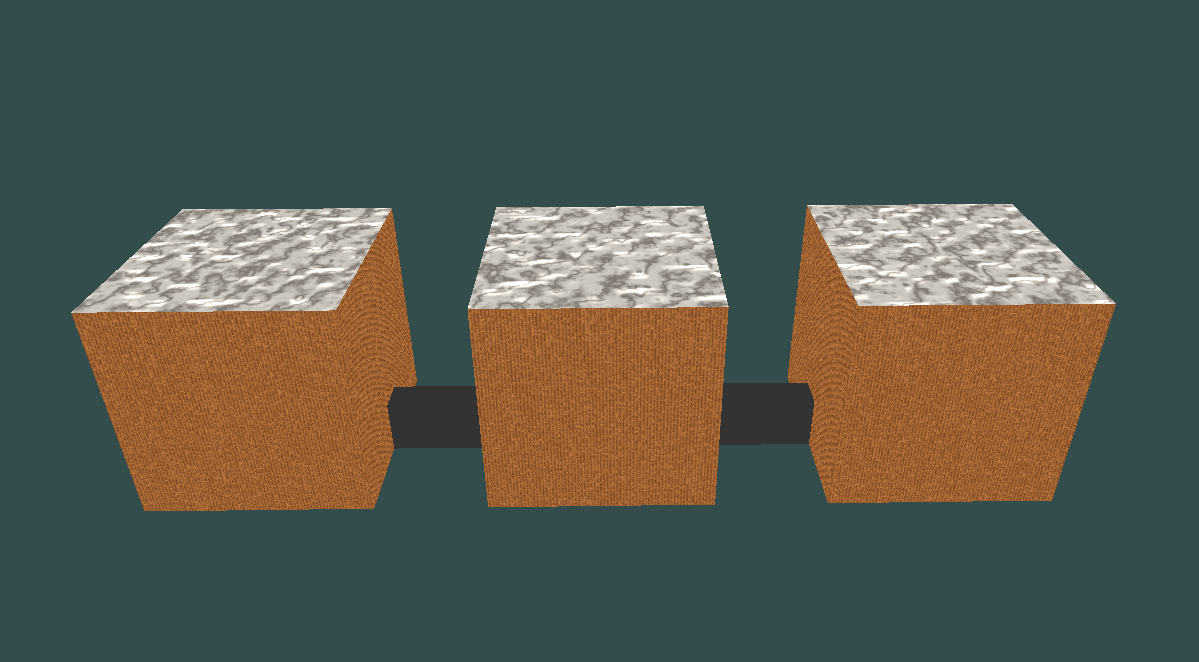
\includegraphics[width=0.8\textwidth]{Images/architecture.png}
    \caption{Structure and architecture of the 3D space as seen from the outside}
\end{figure}

Inside each of the first 2 rooms we can find 3 objects (a sphere, a pyramid and a cube), while in the last room we only find 2 objects of larger dimensions (a sphere and a cube). 
\newline

In the first room we can find Perlin noise applied to all the objects: the sphere has a simple Perlin noise, the cube has Perlin noise with multiple octaves and the pyramid has Perlin Noise with turbulence.
\begin{figure}[H]
    \centering
    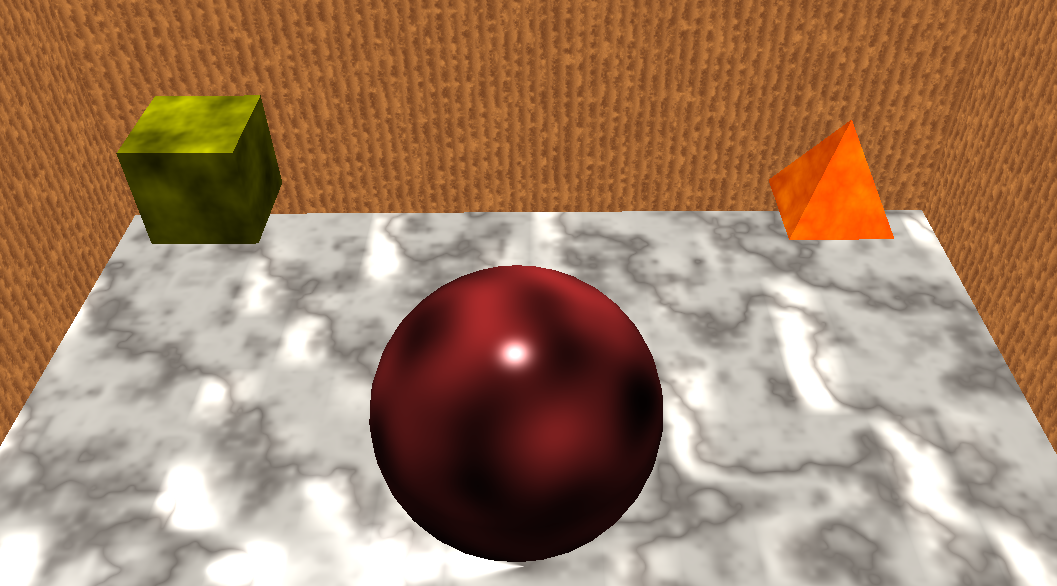
\includegraphics[width=0.8\textwidth]{Images/firstRoom.png}

    \caption{First room}
\end{figure}

In the second room we can find Simplex noise applied to the cube, Multifractal noise applied to the sphere and Cellular noise applied to the pyramid.
\begin{figure}[H]
    \centering
    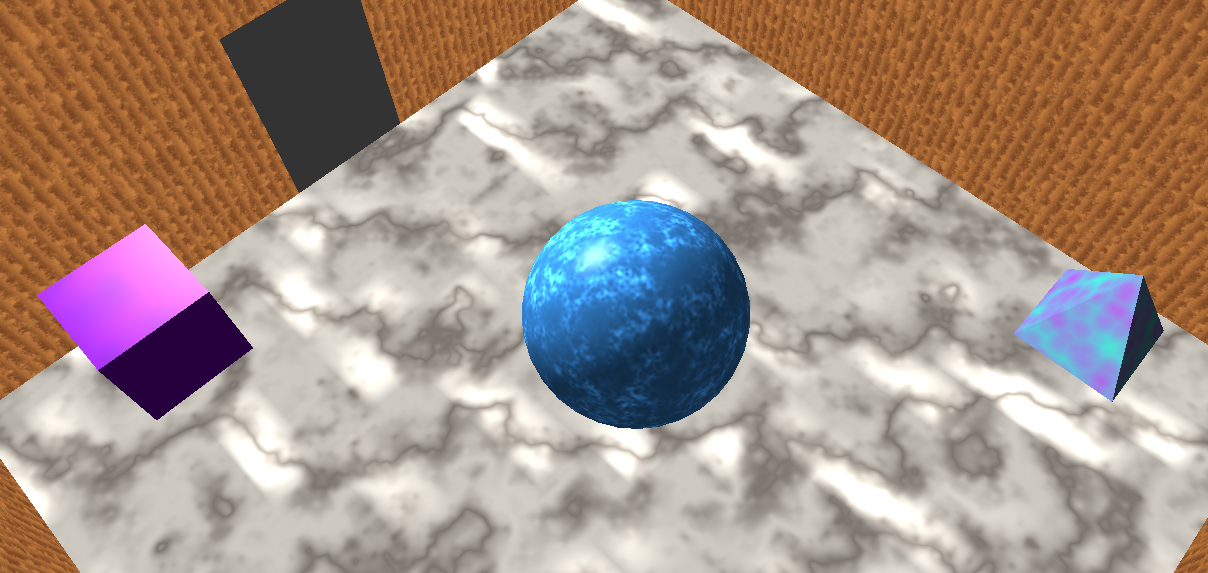
\includegraphics[width=0.8\textwidth]{Images/secondRoom.png}
    \caption{Second room}
\end{figure}

While in the first two rooms all types of noises where applied only to the diffusive color of the objects, 
in the third room we can find Perlin noise applied on the normal map in the case of the sphere, while for the cube the Perlin noise is applied to its transparency.
\begin{figure}[H]
    \centering
    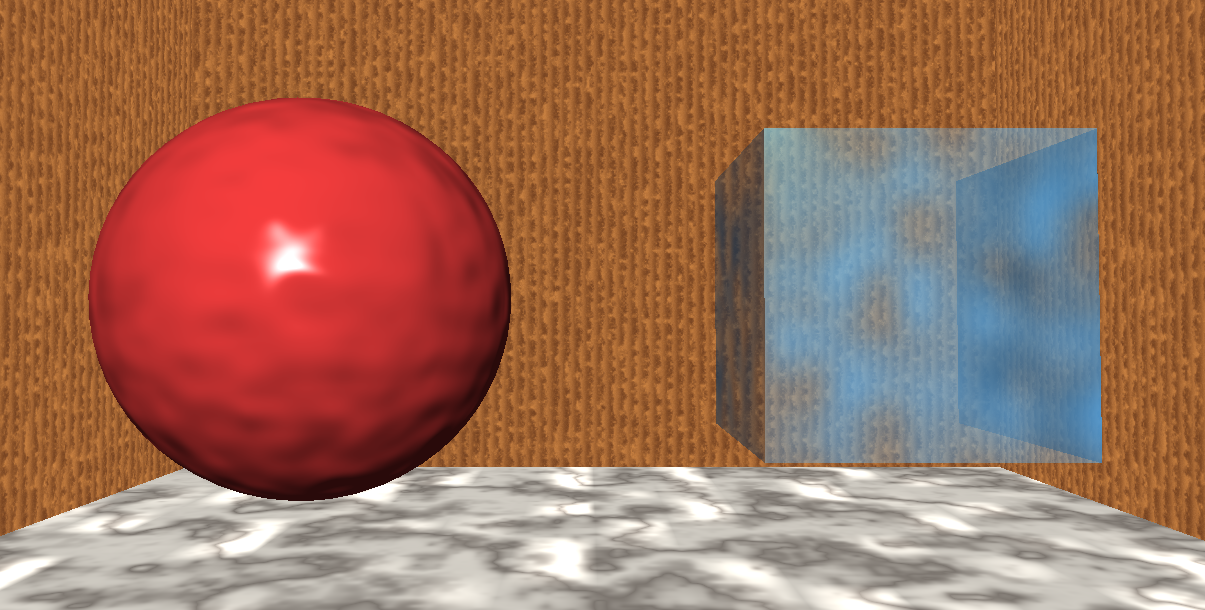
\includegraphics[width=0.8\textwidth]{Images/thirdRoom.png}
    \caption{Third room}
\end{figure}
\subsection {Controls}
The user is able to move and look around in this space by using the WASD keys to move and the mouse to orient the camera. 

\newpage

\section{Algorithms and Techniques}
\label{sec:algorithms}
This section will explain in detail all types of noise utilized and where the user can find them in the project.

\subsection {Noises}
\begin{itemize}
    \item \textbf{Perlin Noise}:
    \newline
    Perlin noise is a gradient noise function that produces smooth, continuous random variations. It is widely used in computer graphics for procedural texture generation due to its natural appearance. 
    The implementation typically involves three steps:
    \begin {enumerate}
        \item \textbf{Grid definition}:
        \newline 
        Define an n-dimensional grid where each grid intersection has associated with it a fixed random n-dimensional unit-length gradient vector.

        \begin{figure}[H]
            \centering
            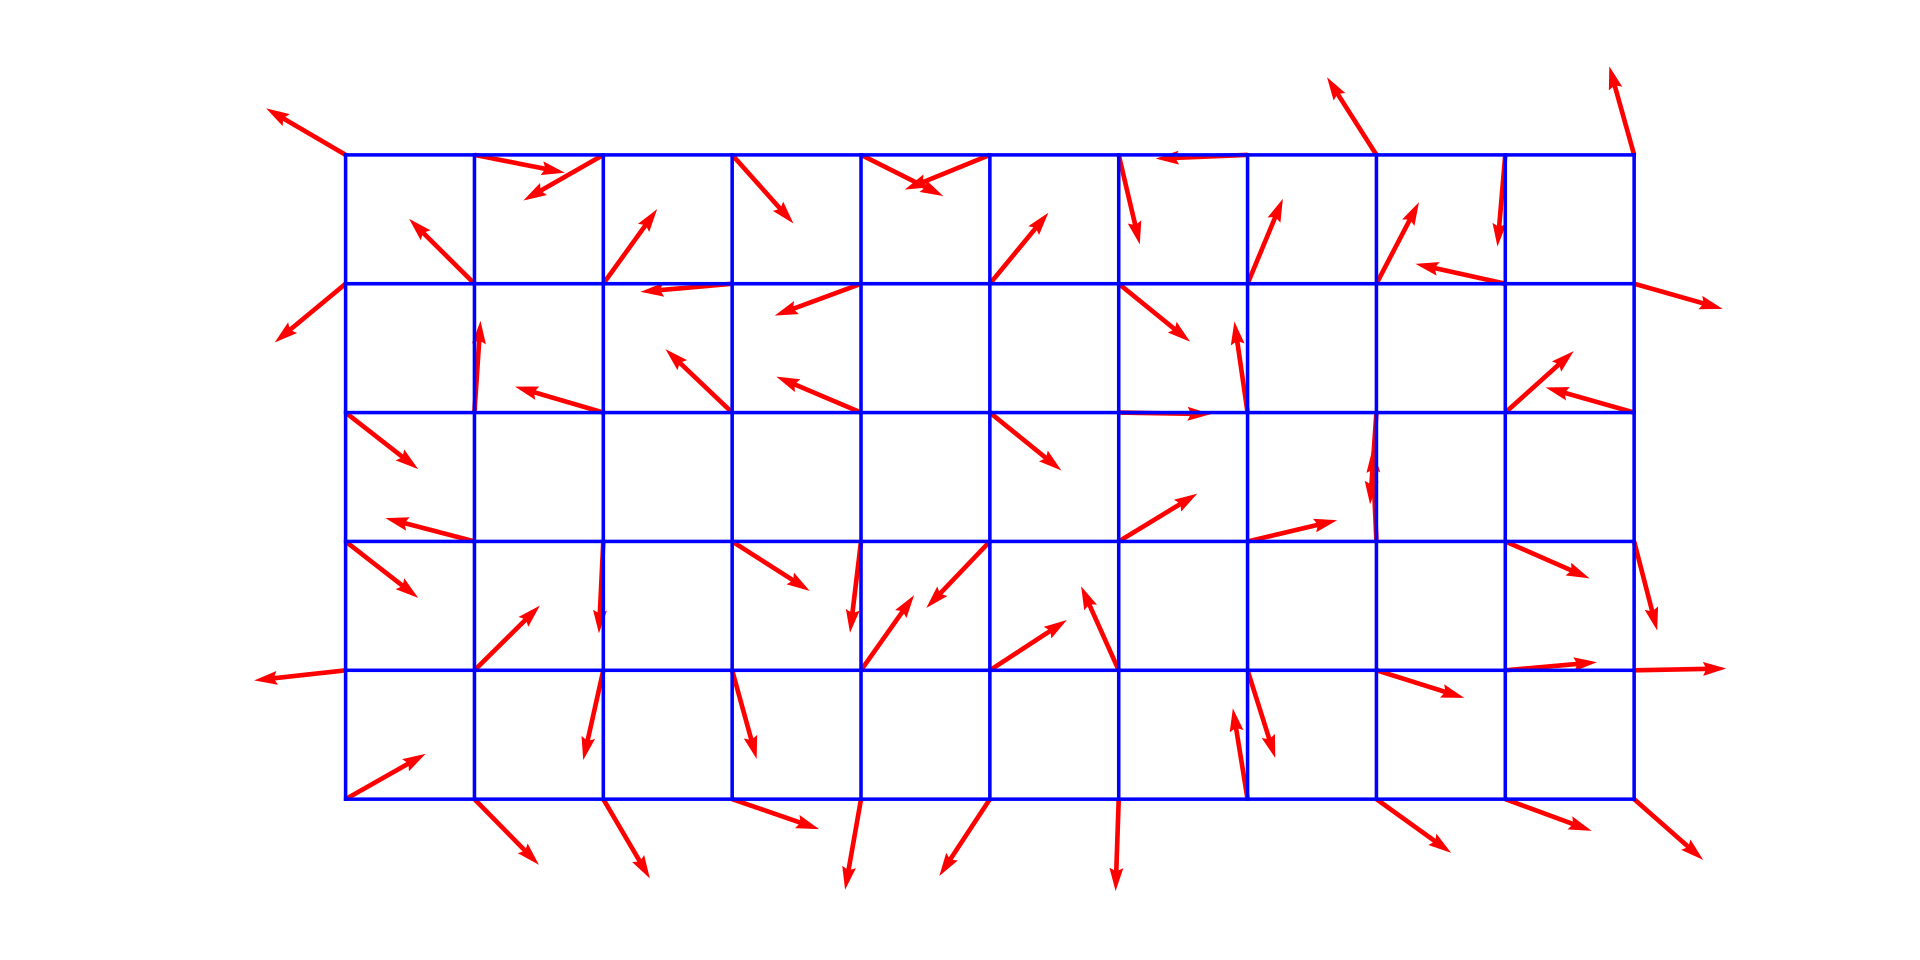
\includegraphics[width=0.8\textwidth]{Images/perlinGrid.png}
        \end{figure}

        \item \textbf{Dot Product}:
        \newline
        For working out the value of any candidate point, first find the unique grid cell in which the point lies. Then, identify the 2n corners of that cell and their associated gradient vectors. 
        Next, for each corner, calculate an offset vector. An offset vector is a displacement vector from that corner to the candidate point.
        For each corner, we take the dot product between its gradient vector and the offset vector to the candidate point. This dot product will be zero if the candidate point is exactly at the grid corner.

        \begin{figure}[H]
            \centering
            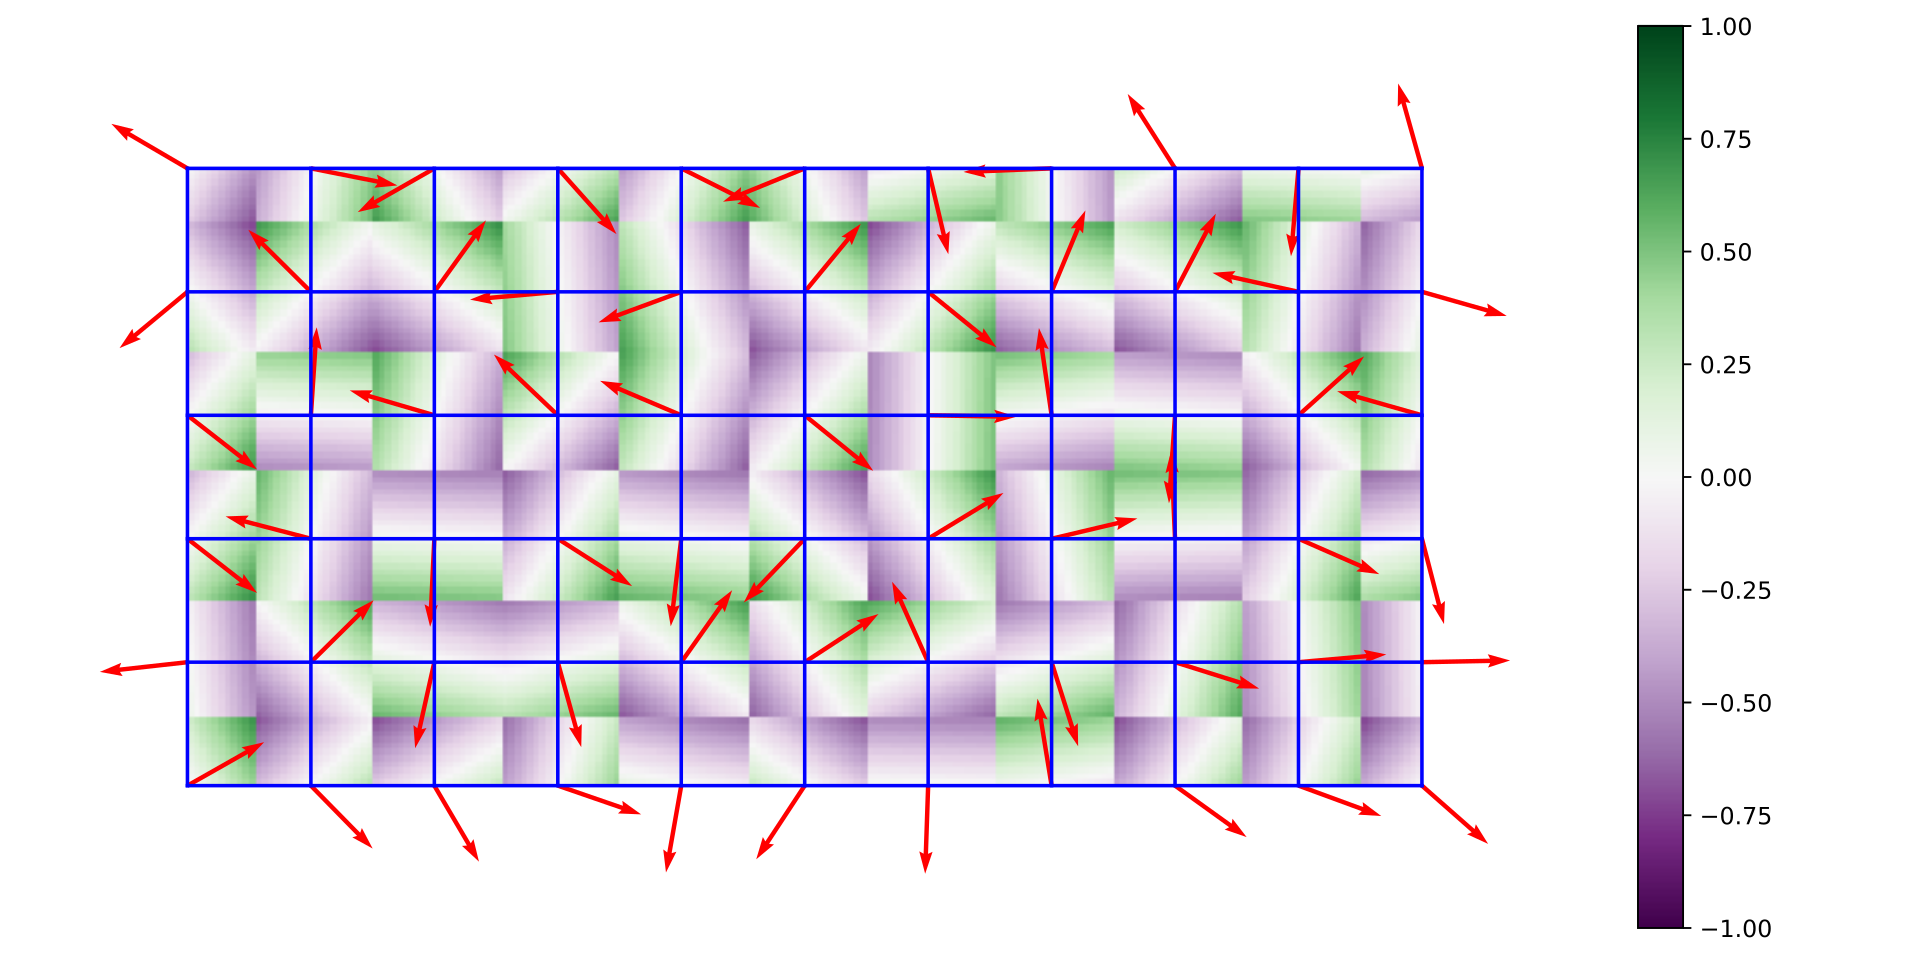
\includegraphics[width=0.8\textwidth]{Images/perlinDot.png}
        \end{figure}

        \item \textbf{Interpolation}:
        \newline
        The final step is interpolation between the 2n dot products. Interpolation is performed using a function that has zero first derivative (and possibly also second derivative) at the 2n grid nodes. 
        Therefore, at points close to the grid nodes, the output will approximate the dot product of the gradient vector of the node and the offset vector to the node. 
        This means that the noise function will pass through 0 at every node, giving Perlin noise its characteristic look.

        \begin{figure}[H]
            \centering
            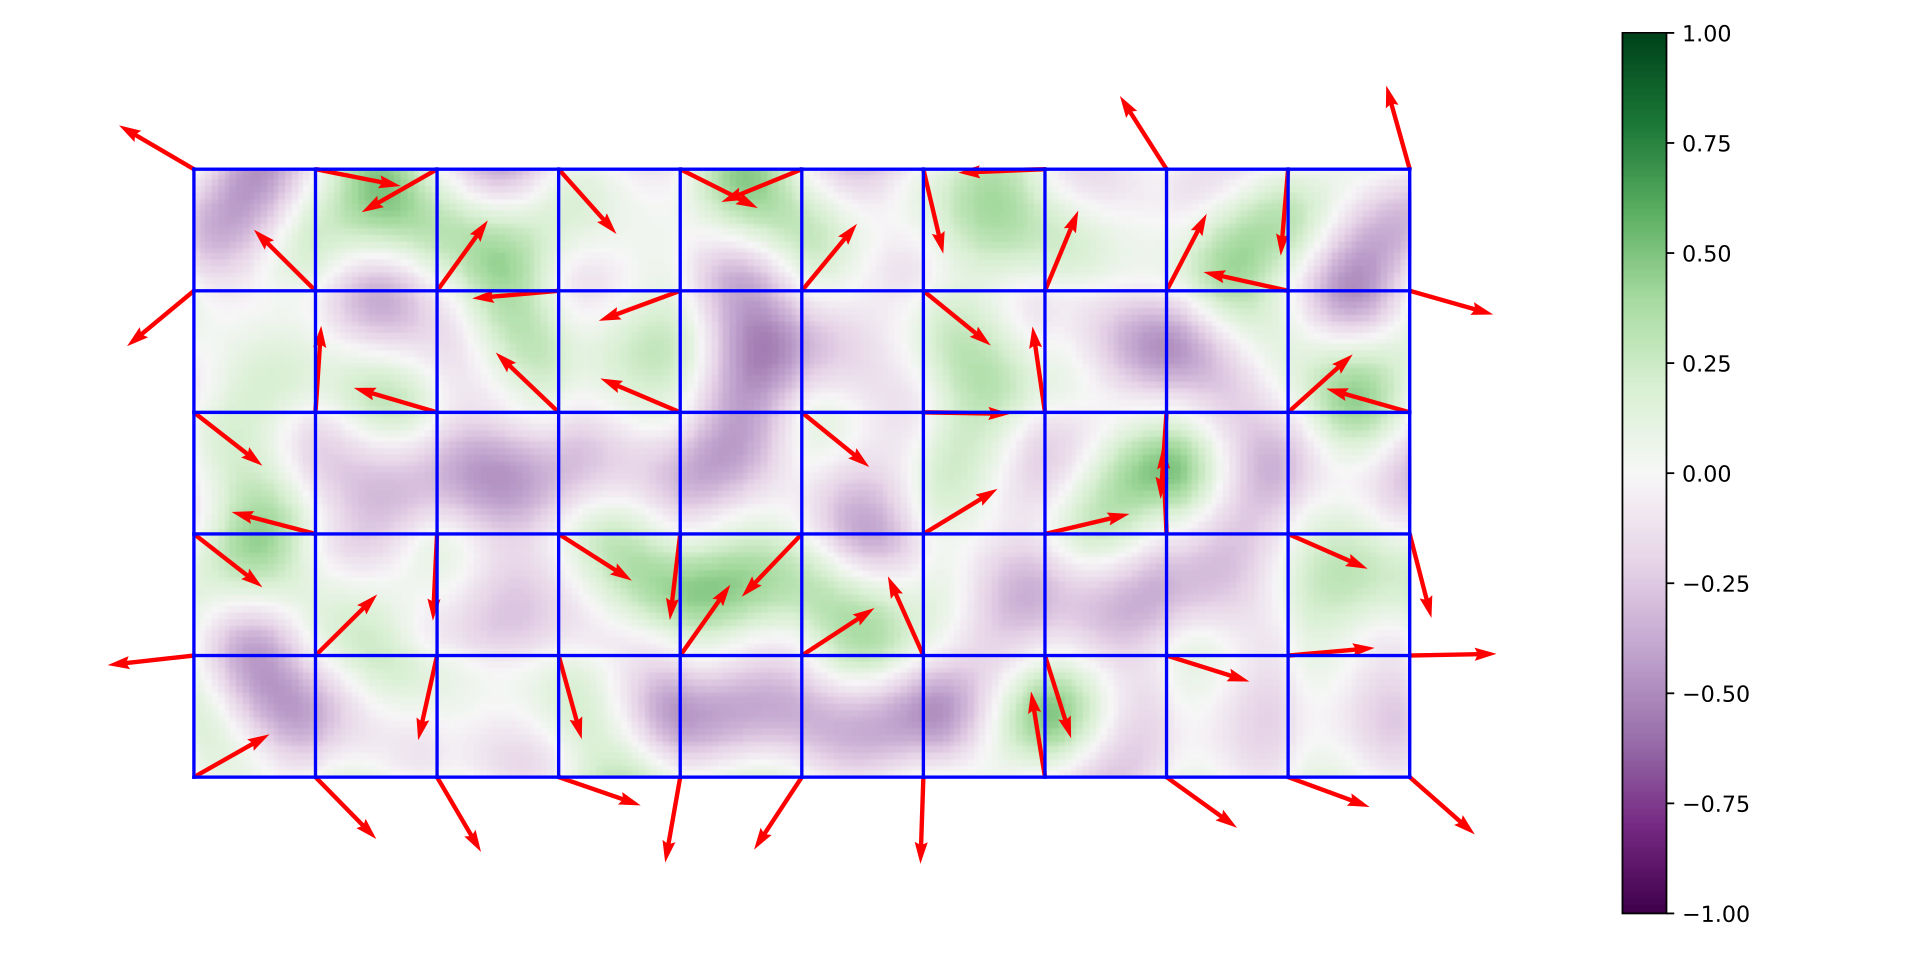
\includegraphics[width=0.8\textwidth]{Images/perlinInterpolation.png}
        \end{figure}
    \end{enumerate}

    \item \textbf{Perlin Noise (with Multiple Octaves)}:
    \newline
    Perlin noise with multiple octaves is a technique that combines multiple Perlin noise functions to create a more complex and detailed noise pattern. 
    It involves summing together multiple octaves of Perlin noise, each octave is a separate layer of noise with a different frequency and amplitude.

    Multiple octaves are combined by adding the noise values from each layer. Typically, the frequency is doubled, and the amplitude is halved for each successive octave. 
    This creates a fractal-like pattern where larger features are overlaid with progressively finer details.

    \textbf{Fractal Brownian Motion (fBm)} is a common technique for combining octaves. It involves summing the noise values from each octave, weighted by their respective amplitudes. 
    The result is a texture that has both large-scale and small-scale variations.

    \item \textbf{Perlin Noise (with Turbulence)}:
    \newline
    Turbulence is a technique used in procedural texture generation to create chaotic, swirling patterns that resemble natural phenomena like smoke, fire, or flowing water. 
    It is a variation of fractal Brownian motion (fBm) that uses the absolute value of noise to produce sharp, jagged features.

    Unlike standard fBm, which sums smooth noise values, turbulence takes the absolute value of each noise layer. 
    This introduces sharp changes and more pronounced variations, which are characteristic of turbulent patterns.

    The final turbulence value is normalized by dividing by the maximum possible value, ensuring it remains within a usable range.

    \item \textbf{Perlin Noise on Normal Map}:
    \newline
    This technique is often used to simulate surface details without the need for additional geometry, enhancing the realism of the rendered object.
    The implementation typically involves three steps:
    \begin {enumerate}
        \item \textbf{Noise Generation}:
        \newline
        Perlin noise is generated based on the fragment position. This noise is used to create small variations in the surface normals.

        \item \textbf{Normal Perturbation}:
        \newline
        The generated noise is used to perturb the original normals. This involves adjusting the normal vectors based on the noise values, simulating a bumpy surface.

        \item \textbf{Lighting Calculations}:
        \newline
        The perturbed normals are then used in the lighting calculations, affecting the diffuse and specular components of the lighting model.   
    \end{enumerate}

    \item \textbf{Perlin Noise on Transparency}:
    \newline
    This technique allows for the simulation of materials with varying opacity, such as frosted glass or organic surfaces.
    The implementation typically involves three steps:
    \begin {enumerate}
        \item \textbf{Noise Generation}:
        \newline
        Perlin noise is generated based on the fragment position. This noise value is used to determine the transparency level of each fragment.

        \item \textbf{Alpha Calculation}:
        \newline
        The noise value is mapped to an alpha value, which controls the transparency of the fragment. This mapping is done using a linear interpolation between minimum and maximum alpha values.

        \item \textbf{Fragment Color Output}:
        \newline
        The calculated alpha value is combined with the base color and lighting calculations to produce the final fragment color, including its transparency.
    \end{enumerate}

    \item \textbf{Simplex Noise}:
    \newline
    Simplex noise is a type of gradient noise that improves upon classic Perlin noise by reducing directional artifacts and computational complexity. 
    It is particularly useful for generating smooth, organic textures in graphics applications.
    The implementation typically involves five steps:

    \begin {enumerate}  
        \item \textbf{Coordinate Skewing}:
        \newline
        Simplex noise uses a skewed grid to reduce the number of required gradient calculations.

        \begin{figure}[H]
            \centering
            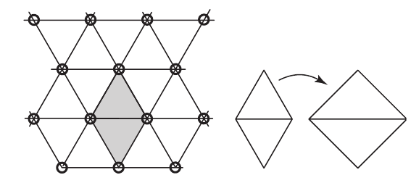
\includegraphics[width=0.8\textwidth]{Images/simplexGrid.png}
            \caption{Skewed grid in 2D, made of triangles}
        \end{figure}

        \item \textbf{Simplicial Subdivision}:
        \newline
        The grid is divided into simplices (triangles in 2D, tetrahedra in 3D), which are the smallest possible convex shapes that can fill the space without gaps or overlaps.

        \item \textbf{Gradient Selection}:
        \newline
        For each simplex, a random gradient vector is assigned to each of its vertices. These gradients are used to determine the direction of the noise variations.

        \item \textbf{Interpolation}:
        \newline
        The noise values at the corners are interpolated using a smooth function to ensure continuous transitions across the grid.

        \item \textbf{Normalization}:
        \newline
        The final noise value is normalized to ensure it remains within a usable range.
    \end{enumerate}

    \item \textbf{Multifractal Noise}:
    \newline
    Multifractal noise is a complex noise function that combines multiple layers of noise with varying parameters to create highly detailed and intricate textures.
    It is particularly useful for simulating natural phenomena that exhibit self-similar patterns, such as landscapes, clouds, and other organic structures.
    Multifractal noise is characterized by its self-similar nature, where patterns repeat at different scales. This is achieved by layering multiple octaves of noise, each with a different frequency and amplitude.

    Unlike standard fBm, where amplitude and frequency are fixed for each octave, multifractal noise adjusts these parameters dynamically based on the current noise value. 
    This creates a more complex and varied texture.

    The contribution of each octave is weighted by the current noise value, which influences the amplitude of subsequent octaves. 
    This weighting creates a feedback loop that enhances the self-similar nature of the texture.

    \textbf{Parameters}:
    Aside for the number of octaves, there are 2 more parameters that influence the Multifractal Noise:
    \begin{itemize}
        \item \textbf{Lacunarity}:
        \newline
        Lacunarity controls the frequency scaling between octaves. Higher lacunarity results in more frequent changes in detail.

        \item \textbf{Hurst Exponent (H)}:
        \newline
        The Hurst Exponent determines the fractal dimension of the noise. Higher values of H result in smoother, more persistent patterns.       
    \end{itemize}

    \begin{figure}[H]
        \centering
        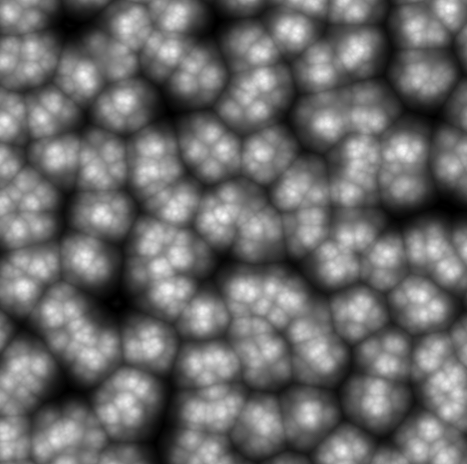
\includegraphics[width=0.7\textwidth]{Images/multifractal.png}
        \caption{Example of multifractal noise}
    \end{figure}   

    \item \textbf{Cellular Noise}:
    \newline
    Cellular noise, also known as Worley noise, is a type of procedural texture that generates patterns based on the distance to the nearest feature point in a grid. 
    It is often used to create textures that resemble natural cellular structures, such as stone, skin, or organic patterns.
    The implementation typically involves four steps:

    \begin{enumerate}
        \item \textbf{Grid Definition}:
        \newline
        The grid is defined as a regular grid of points in the space.

        \item \textbf{Feature Point Generation}:    
        \newline
        A set of feature points are randomly distributed throughout the grid. These points act as the centers of the cellular structure.

        \item \textbf{Distance Calculation}:
        \newline
        For each point in the grid, the distance to the nearest feature point is calculated. The minimum distance determines the noise value at that point.   

        \item \textbf{Normalization}:
        \newline
        The final noise value is normalized to ensure it remains within a usable range.
    \end{enumerate}
    
    The resulting noise pattern consists of cells, where each cell is centered around a feature point. The edges of the cells are defined by the equidistant lines between neighboring feature points.

    \begin{figure}[H]
        \centering
        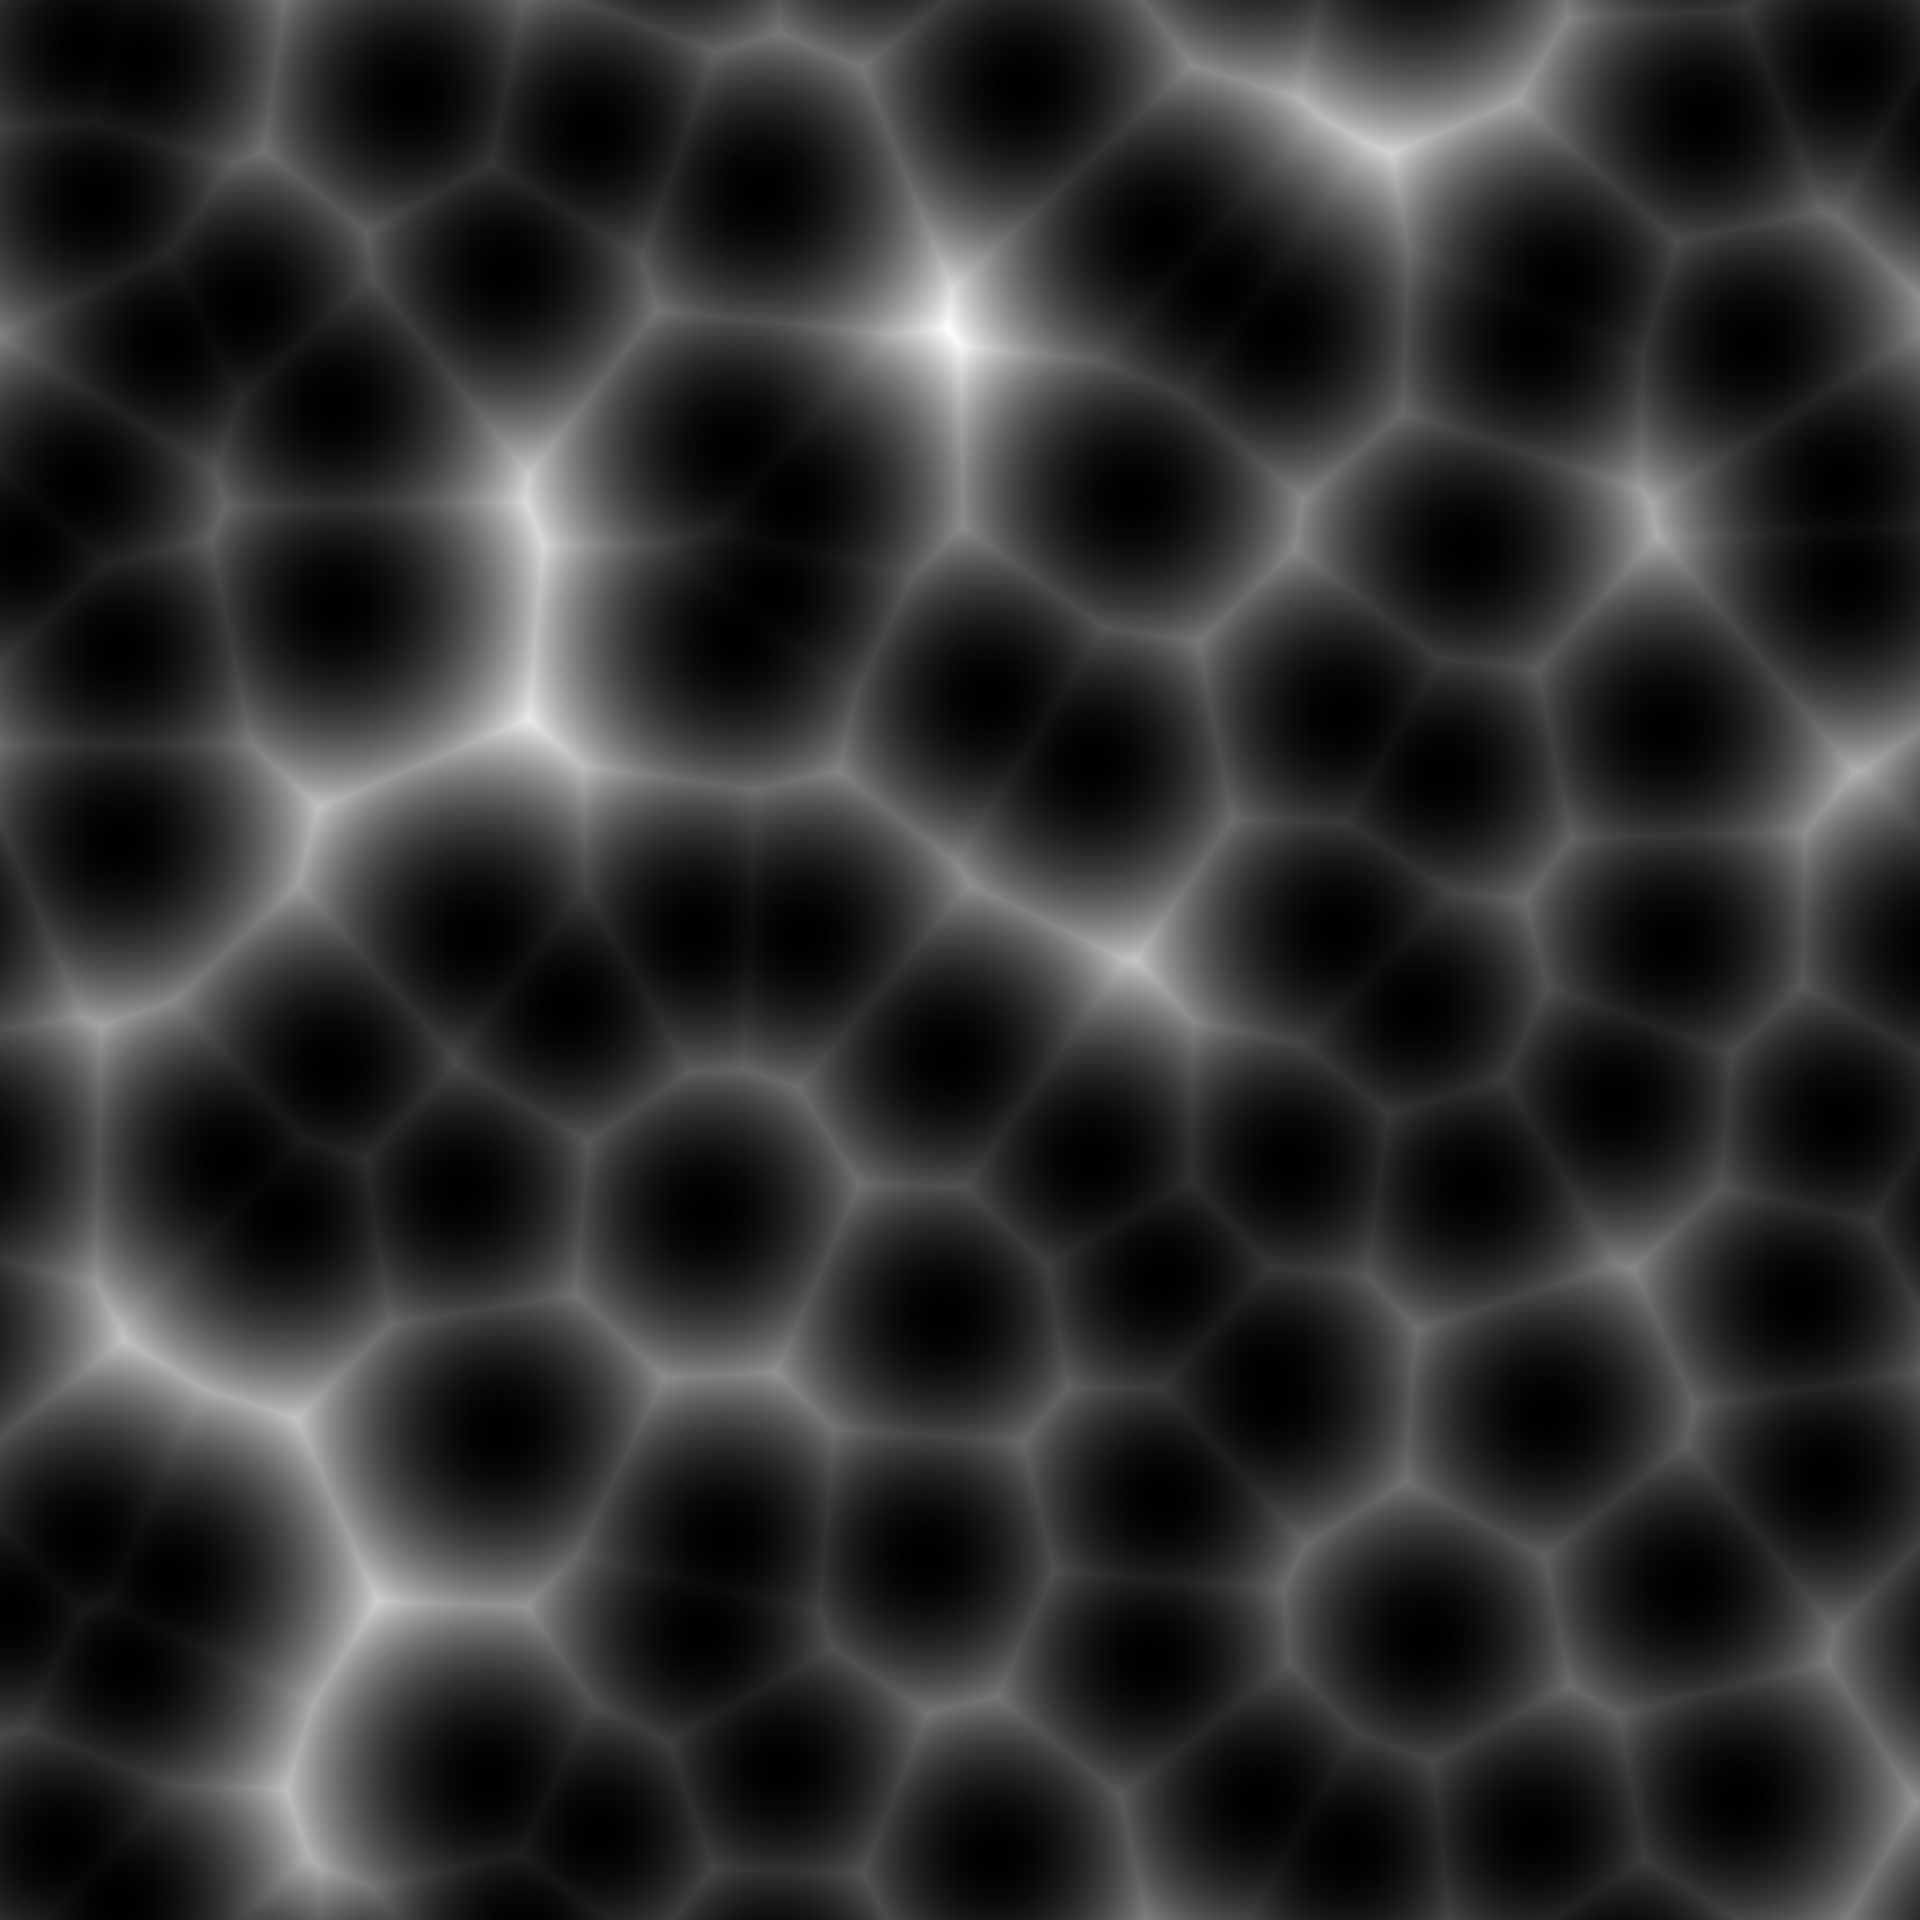
\includegraphics[width=0.7\textwidth]{Images/cellular.png}
        \caption{Example of cellular noise}
    \end{figure} 
    
\end{itemize}

\newpage

\section{Implementation Details}
\label{sec:implementation}
In this section are reported all the most relevant sections of the code, with particular focus on the noise generation and the shaders.
\newline
\subsection{Noise Generation}
\label{sec:noiseGeneration}

\begin{enumerate}
    \item \textbf{Perlin Noise and variations}:
    \begin{itemize}
        \item \textbf{fragment\_sphere1.glsl}:
        \newline
        This shader is used to render the sphere in the first room, it uses simple Perlin noise to modify the diffusive color of the sphere.

        \begin{figure}[H]
            \label{img:noiseFunction}
            \centering
            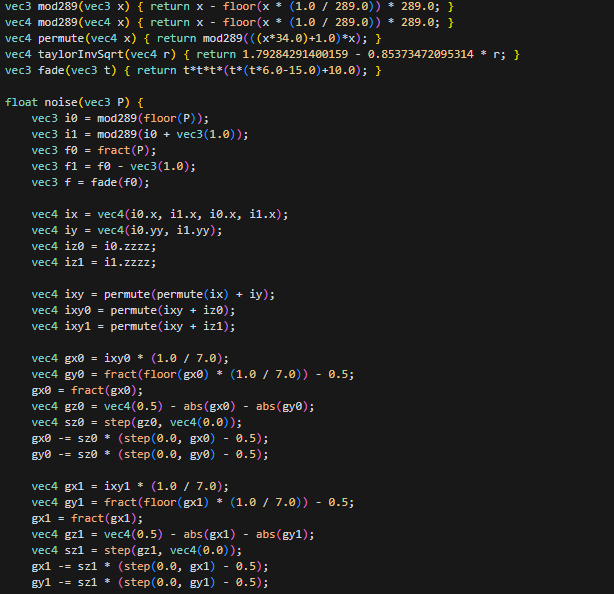
\includegraphics[width=1\textwidth]{Images/sphere1code.png}
        \end{figure}

        \begin{figure}[H]
            \centering
            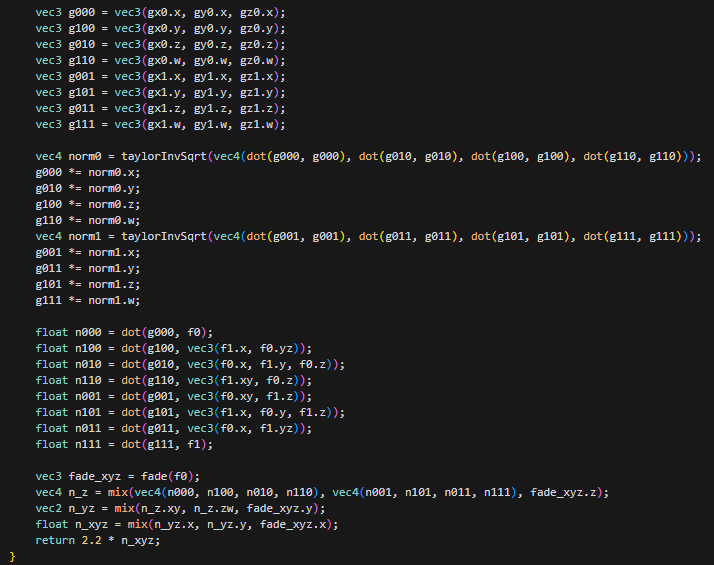
\includegraphics[width=1\textwidth]{Images/sphere1code2.png}
            \caption{snippet of code used to implement Perlin noise}
        \end{figure}

        \textbf{Explanation of the code}:

        \begin{itemize}
            \item \textbf{mod289 and permute}:
            \newline
            These functions are used to wrap indices and generate pseudo-random permutations, ensuring that the noise pattern repeats seamlessly across the grid.

            \item \textbf{taylorInvSqrt}:
            \newline
            This function is used to normalize gradient vectors, ensuring they have unit length, which is crucial for consistent noise values.

            \item \textbf{fade}:
            \newline
            This function is used to interpolate between the noise values at the corners of the grid.        
        \end{itemize}

        The "noise" function proceeds to generate the Perlin noise following the procedure detailed in the section \hyperref[sec:algorithms]{algorithms}.
    \newpage
        
        \item \textbf{fragment\_cube1.glsl}:
        \newline
        This shader is used to render the cube in the first room, it uses Perlin noise with multiple octaves to modify the diffusive color of the cube.

        \begin{figure}[H]
            \centering
            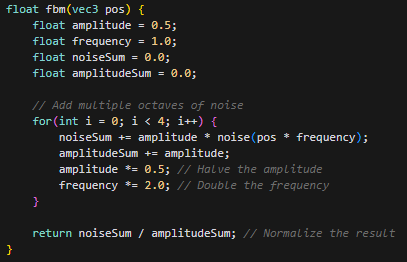
\includegraphics[width=0.8\textwidth]{Images/cube1code.png}
            \caption{snippet of code used to implement Perlin noise with multiple octaves}
        \end{figure}

        \textbf{Explanation of the code}:

        \begin{itemize}
            \item The for loop runs for a specified number of octaves, in this case 4.
            \item For each octave, the noise function is called with the position scaled by the current frequency.
            \item After each octave, the amplitude is halved, and the frequency is doubled.
            \item The final noise value is normalized by dividing by the sum of amplitudes to ensure it remains within a usable range.
        \end{itemize}

        A "noise" function identical to the one seen \hyperref[img:noiseFunction]{before} proceeds to generate the Perlin noise following the procedure detailed in the section \hyperref[sec:algorithms]{algorithms}.

    \newpage

        \item \textbf{fragment\_pyramid1.glsl}:
        \newline
        This shader is used to render the pyramid in the first room, it uses Perlin noise with turbulence to modify the diffusive color of the pyramid.

        \begin{figure}[H]
            \centering
            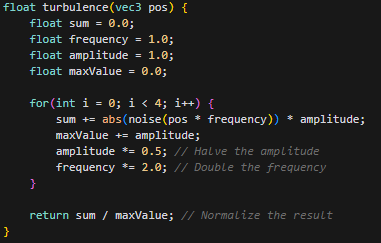
\includegraphics[width=0.8\textwidth]{Images/pyramid1code.png}
            \caption{snippet of code used to implement Perlin noise with turbulence}
        \end{figure}

        \textbf{Explanation of the code}:     

        \begin{itemize}
            \item The for loop runs for a specified number of octaves, in this case 4.
            \item For each octave, the noise function is called with the position scaled by the current frequency. The absolute value of the noise is taken to create sharp features.
            \item After each octave, the amplitude is halved, and the frequency is doubled.
            \item The final turbulence value is normalized by dividing by the sum of amplitudes, ensuring it remains within a consistent range.
        \end{itemize}

        A "noise" function identical to the one seen \hyperref[img:noiseFunction]{before} proceeds to generate the Perlin noise following the procedure detailed in the section \hyperref[sec:algorithms]{algorithms}.
    \end{itemize}


    \newpage

    \item \textbf{Simplex Noise (fragment\_cube2.glsl)}:
    \newline
    This shader is used to render the cube in the second room, it uses Simplex noise to modify the diffusive color of the cube.

    \begin{figure}[H]
        \label{img:snoiseFunction}
        \centering
        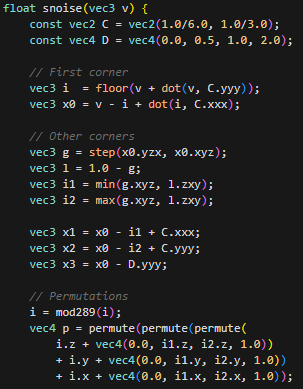
\includegraphics[width=0.8\textwidth]{Images/cube2code.png}
    \end{figure}

    \begin{figure}[H]
        \centering
        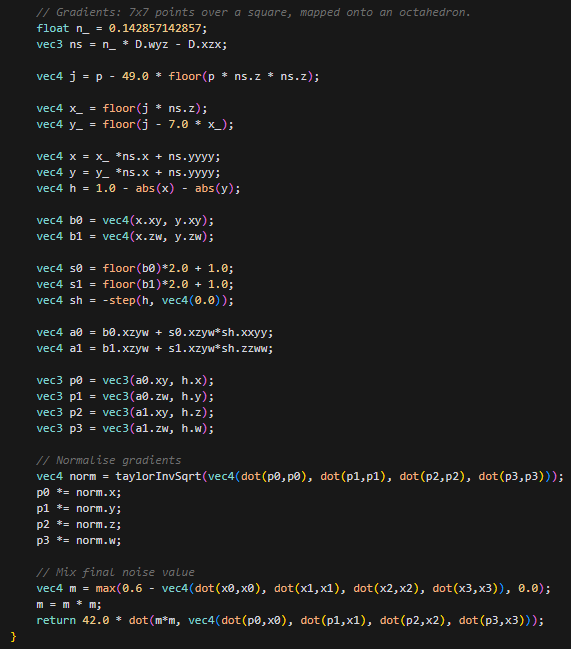
\includegraphics[width=0.9\textwidth]{Images/cube2code2.png}
        \caption{snippet of code used to implement Simplex noise}
    \end{figure}

    \textbf{Explanation of the code}:
    \begin {itemize}
        \item The input vector v is skewed to determine the simplex cell it falls into, the corners of the simplex are then calculated.
        \item Gradients are calculated at each corner of the simplex, these gradients are used to compute the influence of each corner on the final noise value.
        \item The final noise value is normalized to ensure it fits within a usable range.
        \item The noise values at the corners are interpolated using a smooth function to ensure continuous transitions.    
    \end{itemize}

    \newpage

    \item \textbf{Multifractal Noise (fragment\_sphere2.glsl)}:
    \newline
    This shader is used to render the sphere in the second room, it uses Multifractal noise to modify the diffusive color of the sphere.

    \begin{figure}[H]
        \centering
        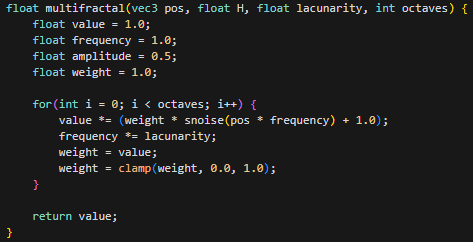
\includegraphics[width=0.8\textwidth]{Images/sphere2code.png}
        \caption{snippet of code used to implement Multifractal noise}
    \end{figure}

    \textbf{Explanation of the code}:
    \begin {itemize}
        \item The function starts with an initial value of 1.0, and sets the initial frequency and amplitude.
        \item The loop iterates over the specified number of octaves.
        \item For each octave, the simplex noise function snoise is called with the position scaled by the current frequency. 
            The result is adjusted by the current weight and added to the value.  
        \item The frequency is multiplied by the lacunarity to increase the detail for the next octave. 
            The weight is updated based on the current value and clamped to ensure it remains within a valid range.
        \item The final multifractal noise value is returned, representing the combined effect of all octaves.
    \end{itemize}

    A "snoise" function identical to the one seen \hyperref[img:snoiseFunction]{before} proceeds to generate the Simplex noise.

    \newpage

    \item \textbf{Cellular Noise (fragment\_pyramid2.glsl)}:
    \newline
    This shader is used to render the pyramid in the second room, it uses Cellular noise to modify the diffusive color of the pyramid.      
    
    \begin{figure}[H]
        \centering
        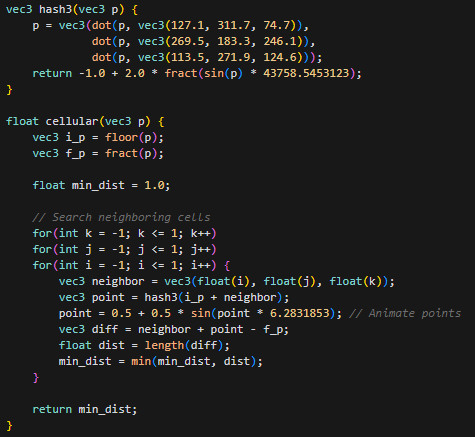
\includegraphics[width=0.9\textwidth]{Images/pyramid2code.png}
    \end{figure}

    \begin{figure}[H]
        \centering
        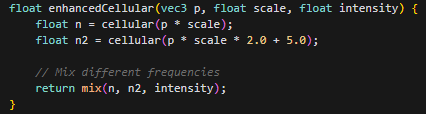
\includegraphics[width=0.9\textwidth]{Images/pyramid2code2.png}
        \caption{snippet of code used to implement Cellular noise}
    \end{figure}
    
\newpage

    \textbf{Explanation of the code}:
    \begin {itemize}

        \item \textbf{hash3}:
        \newline
        The hash3 function generates pseudo-random feature points within each grid cell. It uses a combination of dot products and trigonometric functions to ensure randomness.

        \item \textbf{cellular}:
        \newline
        The input position p is split into its integer (i\_p) and fractional (f\_p) parts. The integer part identifies the grid cell, while the fractional part is used to calculate distances within the cell.
        The shader iterates over neighboring cells to find the nearest feature point: the distance to each feature point is calculated, and the minimum distance is stored.
        The feature points are animated by applying a sine function, which can create dynamic patterns over time.

        \item \textbf{enhancedCellular}:
        \newline
        The function generates two layers of cellular noise at different scales, this layering adds complexity and detail to the texture. 
        The two noise layers are mixed together using a specified intensity, this allows for blending between the different scales of noise, creating a more intricate pattern.
    \end{itemize}

\newpage
    
    \item \textbf{Perlin Noise on Normal Map (fragment\_sphere3.glsl)}:
    \newline
    This shader is used to render the sphere in the third room, it uses Perlin noise to modify the normal map of the sphere.

    \begin{figure}[H]
        \centering
        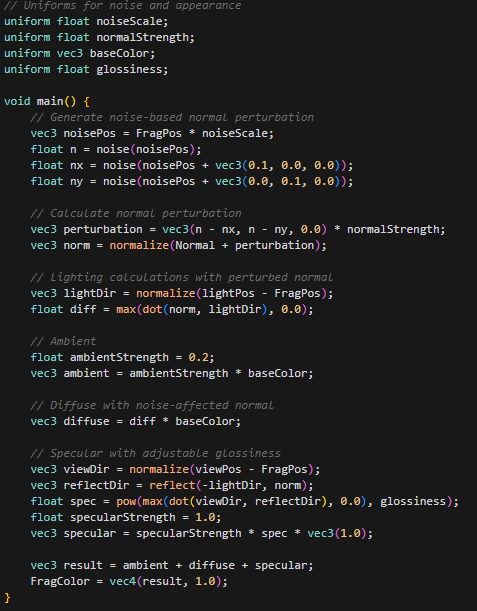
\includegraphics[width=0.8\textwidth]{Images/sphere3code.png}
        \caption{snippet of code used to implement Perlin noise on normal map}
    \end{figure}

    \textbf{Explanation of the code}:
    \begin {itemize}
        \item \textbf{Noise Generation}:
        \newline
        The position FragPos is scaled by noiseScale to control the frequency of the noise. The noise function is called to generate noise values at the current position and slightly offset positions (nx and ny).

        \item \textbf{Normal Perturbation}:
        \newline
        The difference between the noise values (n - nx and n - ny) is used to create a perturbation vector. This vector is scaled by normalStrength to control the intensity of the normal perturbation.
        The original normal Normal is adjusted by adding the perturbation vector, and the result is normalized to ensure it remains a unit vector.

        \item \textbf{Lighting Calculations}:
        \newline
        The perturbed normal norm is used in the lighting calculations, this affects the diffuse and specular components, creating the appearance of a textured surface.
        The diffuse component is calculated using the dot product of the perturbed normal and the light direction.
        The specular component is calculated using the reflection of the light direction around the perturbed normal, with the glossiness controlling the sharpness of the specular highlight.
    \end{itemize}
    
    A "noise" function identical to the one seen \hyperref[img:noiseFunction]{before} proceeds to generate the Perlin noise following the procedure detailed in the section \hyperref[sec:algorithms]{algorithms}.

    \newpage

    \item \textbf{Perlin Noise on Transparency (fragment\_cube3.glsl)}:
    \newline
    This shader is used to render the cube in the third room, it uses Perlin noise to modify the transparency of the cube.

    \begin{figure}[H]
        \centering
        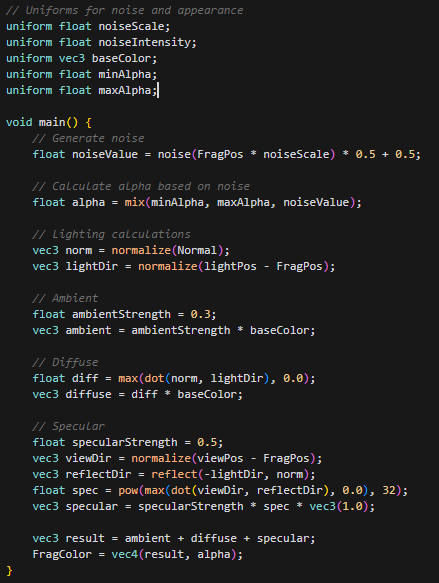
\includegraphics[width=0.8\textwidth]{Images/cube3code.png}
        \caption{snippet of code used to implement Perlin noise on transparency}
    \end{figure}

    \textbf{Explanation of the code}:
    \begin {itemize}
        \item \textbf{Noise Generation}:
        \newline
        The position FragPos is scaled by noiseScale to control the frequency of the noise. The noise function is called to generate a noise value, which is normalized to the range [0, 1] by multiplying by 0.5 and adding 0.5.

        \item \textbf{Alpha Calculation}:
        \newline
        The mix function is used to interpolate between minAlpha and maxAlpha based on the noise value. 
        This determines the transparency level of the fragment, with higher noise values resulting in higher transparency (or vice versa, depending on the values of minAlpha and maxAlpha).

        \item \textbf{Lighting Calculations}:
        \newline
        The base color and lighting calculations (ambient, diffuse, and specular) are performed as usual, using the normalized normal vector and light direction.

        \item \textbf{Fragment Color Output}:
        \newline
        The final fragment color is constructed using the calculated lighting components and the interpolated alpha value. 
        The FragColor output includes the RGB color and the alpha transparency.
    \end{itemize}

    A "noise" function identical to the one seen \hyperref[img:noiseFunction]{before} proceeds to generate the Perlin noise following the procedure detailed in the section \hyperref[sec:algorithms]{algorithms}.

\subsection{Main code}
This section is a short summary that explains how the code in the main file Rooms.cpp is structured:

\begin{itemize}
    \item \textbf{Global Variables}:
    \newline
    Camera and movement variables are defined to control the user's view and navigation through the 3D space.
    Shader program IDs are stored for different objects (cubes, spheres, pyramids) in each room.

    \item \textbf{Noise Parameters}:
    \newline
    Parameters for different noise types (Perlin, Simplex, Multifractal, Cellular) are defined for each room.

    \item \textbf{Shader Setup}:
    \newline
    A function readShaderFile is provided to read shader source code from files, which is then used to compile and link shader programs.

    \item \textbf{Input Handling}:
    \newline
    Functions like "mouse\_callback" and "processInput" handle user input for camera movement and interaction, such as toggling mouse capture and moving the camera with keyboard keys.

    \item \textbf{Object Setup and Rendering}:
    \newline
    Functions are defined to set up vertex data and buffers for different objects (cubes, spheres, pyramids), rooms and corridors. These functions also compile and link shaders for rendering.
    Rendering functions use the shader programs to draw objects with the specified noise parameters and transformations.

    \item \textbf{Cleanup}:
    \newline
    Cleanup functions are provided to delete OpenGL resources (VAOs, VBOs, EBOs, shader programs) when they are no longer needed.

    \item \textbf{ImGui Rendering functions}:
    \newline
    The "renderNoiseControls" function is used to render the ImGui window, which contains the noise parameters for each room.

    \item \textbf{Main Function}:
    \newline
    The main function initializes the application, creates a window, and enters the main loop, which continues until the window is closed, it also handles the loop, updating the view and projection matrices, and rendering the GUI and the 	    objects using the various functions described in details \hyperref[sec:noiseGeneration]{here} in each room.
    In the end, it cleans up the resources calling the apposite functions and exits the program.
\end{itemize}
\end{enumerate}

\section{Conclusions}
\label{sec:conclusions}
The project is a simple but effective way to show and understand how noise can be used to modify the appearance of objects in a 3D scene in a OpenGL context.
It also showcases the various properties, advantages and disadvantages of the different noise types, and how they can be used to create different effects.
\newline
Compagnoni Alessandro, 2025
\end{document}